%-------------------------------------------------------------------------------
%                            BAB II
%               TINJAUAN PUSTAKA DAN DASAR TEORI
%-------------------------------------------------------------------------------
\fancyhf{} 
\fancyfoot[C]{\thepage}
\chapter{TINJAUAN KEPUSTAKAAN}

\par Untuk mendukung penelitian ini, maka dalam bab ini akan dikemukakan beberapa rumusan teori pendukung, yang dikutip dari berbagai referensi baik dalam bentuk buku, artikel, maupun tulisan karya ilmiah lainnya termasuk hasil penelitian sebelumnya yang ada kaitannya dengan penelitian yang dilakukan.

\section{\textit{Indoor Positioning System}}
\textit{Indoor Positioning System} (IPS, atau \textit{"Indoor Location System"}) merupakan teknologi yang menyediakan informasi bagi pengguna berdasarkan lokasi pengguna di dalam sebuah gedung \citep{brena2017evolution}. IPS merupakan proses mendapatkan perangkat atau lokasi pengguna di dalam ruangan atau lingkungan \citep{zafari2019survey}. Banyak penelitian yang dilakukan dalam mengimplementasi IPS dengan berbagai pemanfaatan seperti WLAN. Namun pemanfaatan WLAN memiliki konsumsi daya yang boros pada smartphone sehingga pada akhirnya implementasi IPS diterapkan pada \textit{Bluetooth low Energy} (BLE) yang memiliki konsumsi daya yang lebih rendah. Metode yang dapat dilakukan dalam pengimplementasian IPS adalah metode \textit{trilateration} (berdasarkan jarak), \textit{triangulation} (berdasarkan sudut) dan \textit{fingerprinting} \citep{puspitasari2020}.

\par Pada luar ruangan untuk mendeteksi suatu lokasi sudah diterapkan dengan adanya teknologi GPS, di mana GPS banyak memberikan dampak yang luar biasa pada kehidupan sehari-hari. Namun kegunaan GPS atau sistem lokasi berbasis satelit hanya terbatas pada lingkungan di luar ruangan. Dengan demikian dibutuhkan suatu metode dan teknologi khusus untuk sistem lokasi pada dalam ruangan yang disebut sebagai \textit{Indoor Positioning System} (IPS) \citep{brena2017evolution}. Dengan menggunakan sensor dan teknologi komunikasi sistem penentuan posisi pada IPS dapat menemukan objek di lingkungan dalam ruangan. Peluang pasar pada penggunaan IPS cukup besar sehingga dapat menarik minat ilmiah komunikasi untuk menerapkan teknologi tersebut \citep{brena2017evolution}.

\par Pada teknologi IPS memiliki beberapa pendekatan yaitu, menentukan posisi dengan berbasis WiFi (WPS), menentukan posisi berbasis \textit{Bluetooth Low Energy} (BLE), menentukan posisi berbasis Identifikasi Frekuensi Radio (RFID) dan menentukan posisi dengan menggunakan teknologi \textit{Ultra-Wide Band} (UWB) atau \textit{Visible Light Communication} (VLC) \citep{canton2017bluetooth}. IPS juga dapat dipadukan dengan kemampuan \textit{route guidance} atau pemandu rute serta didampingi dengan sistem pemandu dengan suara.


\section{\textit{Route Guidance System / Wayfinding and Navigation System}}
Menurut \citep{karimi2015indoor}, \textit{Wayfinding and navigation system} memiliki 2 makna, yaitu merupakan perangkat khusus yang menyediakan solusi pencarian jalan dan navigasi tanpa memerlukan tautan komunikasi atau koneksi ke sistem lain dan tanpa penyedia pihak ketiga. Makna ke dua adalah referensi layanan melalui \textit{smartphone} yang menyediakan solusi pencarian arah dan navigasi hanya melalui tautan komunikasi kabel-nirkabel ke sistem jarak jauh yang didukung oleh penyedia pihak ketiga. Dari perspektif komputasi, \textit{Wayfinding and navigation system} adalah platform terpusat, terdistribusi, dan didistribusikan melalui klien (pada \textit{smartphone}) dan server yang dikelola oleh penyedia layanan.

\section{Kalman Filter}
Kalman Filter adalah seperangkat persamaan matematika yang menyediakan cara komputasi yang efisien untuk memperkirakan keadaan suatu proses, dengan cara meminimalkan rata-rata kesalahan kuadrat. Filter ini sangat berguna dalam beberapa aspek: mendukung estimasi-estimasi keadaan lampau, sekarang dan masa depan, dan dapat melakukannya bahkan ketika sifat pasti dari sistem yang dimodelkan tidak diketahui(Welah, 2021). Kalman Filter sendiri merupakan algoritma yang menggunakan serangkaian data yang diamati dari waktu ke waktu, yang mengandung noise dan ketidakakuratan lainnya, untuk memperkirakan variabel yang tidak diketahui dengan lebih akurat. Ini diusulkan oleh R. E. Kalman pada tahun 1960, dan menjadi pendekatan standar untuk estimasi yang optimal. Karena memiliki keunggulan waktu secara realtime, cepat, efisien, dan anti-interferensi yang kuat, Kalman filter telah banyak diterapkan di bidang perhitungan orbit, pelacakan target dan navigasi (Qiang dkk., 2015).

\section{\textit{Fingerprinting}}
Fingerprinting adalah teknik untuk menentukan lokasi dengan pemanfaatan Radio Signal Strength (RSS) dari suatu Access Point (AP). Menurut Yudha dkk. (2018), metode ini memperhitungkan atenuasi karena kekuatan sinyal sering berubah-ubah. Setiap titik reverensi dikumpulkan yang mengintegrasikan adanya penghalang antara transmitter dan receiver.

\par Transmitter untuk teknologi IPS yang ditunjukan untuk WLAN disebut dengan AP, sedangkan transmitter untuk teknologi IPS yang ditunjukan untuk Bluetooth Low Energy disebut dengan Beacon (Puspitasari, 2020). Metode fingerprinting berbasis IPS ini terdiri dari 2 tahap. Tahap pertama adalah tahap pembelajaran (offline), di mana lokasi fingerprints itu sendiri diperoleh dengan cara mengumpulkan RSSI dalam satuan desibel (dB) yang dipancarkan dari masing-masing AP. Kemudian gelombang radio yang dipancarkan AP yang diletakkan pada posisi yang telah ditentukan sebelumnya ditangkap oleh smartphone yang terintegrasi dengan WLAN ataupun Bluetooth.

\par Selama tahap pembelajaran lokasi yang tidak diketahui data pembelajarannya kemudian dirujuk sebagai titik referensi estimasi lokasi. Tahap kedua adalah tahap pengujian (online), di mana keakuratan yang dikumpulkan dalam data pembelajaran. Selama tahap pengujian sistem harus memberikan lokasi setiap objek berdasarkan data RSSI yang diamati. Namun, nilai RSSI bisa dipengaruh oleh keadaan lingkungan sekitar yang dapat mengganggu keakuratannya (Subhan dkk., 2011). Menurut Yudha dkk. (2018), metode Fingerprinting berbasis IPS ini melibatkan 2 tahap yang dapat dilihat pada Gambar x.x.

\begin{figure}[H]
\centering
\shadowbox
{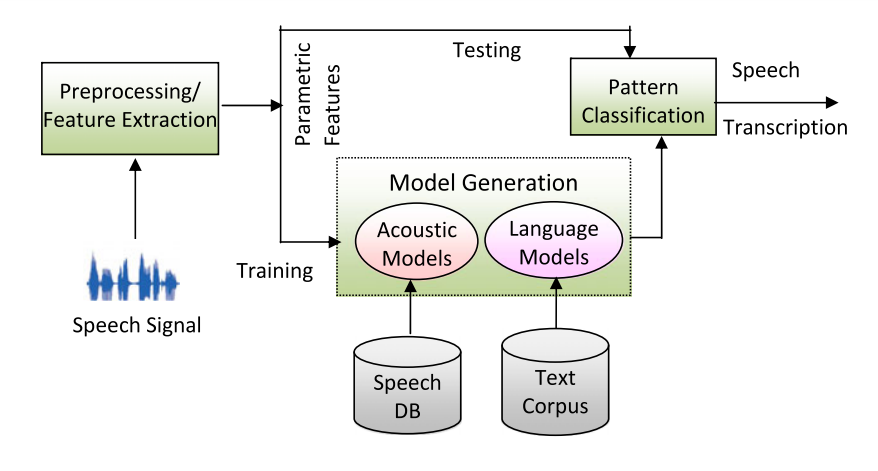
\includegraphics [width = 10cm, height= 5cm]{gambar/sr_arsitektur}}
\caption{Ilustrasi Metode \textit{Fingerprinting} \citep{aggarwal2012}}.
\label{sr_arsitektur}
\end{figure}

\section{\textit{Received Signal Strength Indicator} (RSSI)}
Received Signal Strength Indicator atau RSSI adalah metode pengukuran jarak yang memperoleh sinyal dari transmitter seperti Bluetooth untuk menentukan distance-loss model, dan kemudian memperkirakan posisi pengguna melalui beberapa algoritma (Li dkk, 2018). Menurut Puspitasari (2020) Positioning System menghasilkan data yang penting untuk menghitung lokasi pengguna. Time of Arrival (TOA), Time Difference of Arrival (TDOA), Angle of Arrival (AOA). RSSI memperkirakan jarak node yang belum diketahui ke referensi node dari beberapa kumpulan unit perhitungan dengan menggunakan atenuasi kekuatan sinyal (signal strength) yang dipancarkan oleh transmitter (Puspitasari, 2020).

\par Nilai RSSI didefinisikan dengan bilangan negatif. Semakin tinggi bilangan negatifnya, maka kekuatan sinyal tersebut tergolong lemah. Namun apabila nilainya mendekati 0, maka sinyal tersebut tergolong kuat. RSSI dapat digolongkan menjadi 5 kategori kekuatan sinyal seperti pada Tabel x.x.


\section{\textit{Bluetooth Low Energy)} (BLE)}
Teknologi Bluetooth dikembangkan oleh Ericsson pada tahun 1994 dengan kegunaan sebagai standar komunikasi nirkabel untuk bertukar data dalam jarak dekat (Kaluža, Beg, dab Vukelić, 2017). Teknologi Bluetooth memiliki fitur utama yaitu memiliki biaya yang rendah, konsumsi daya rendah, jangkauan kecil, memiliki ketahanan dan penggunaan secara global. Kecepatan transfer data yang diberikan oleh Bluetooth sebesar 1 Mbit/s dan menggunakan pita frekuensi tanpa izin 2,4 hingga 2,485 GHz (Kaluža, Beg, dan Vukelić, 2017).

\par Pertengahan tahun 2010 spesial otoritas kompeten yang bernama “Bluetooth Special Interest Group" (SIG) mengumumkan spesifikasi Bluetooth 4.0, dimana meliputi : Bluetooth Klasik, Bluetooth dengan kecepatan tinggi, dan protokol Bluetooth hemat energi. Karakteristik dari Bluetooth Low Energy (BLE) adalah memiliki ukuran yang kecil, menggunakan biaya rendah, konsumsi penggunaan daya yang rendah dengan kemungkinan penggunaan sampai beberapa tahun bekerja dengan menggunakan baterai AAA dan memiliki kompatibilitas dengan perangkat seluler, tablet, dan komputer (Kaluža, Beg, dan Vukelić, 2017).



\section{\textit{Beacon}}
BLE memancarkan sinyal dari alat transmitter yang beroperasi menggunakan baterai. Alat transmitter tersebut disebut dengan Beacon. Beacon merupakan alat pendeteksi lokasi dengan harga yang terjangkau, ukurannya yang kecil, memiliki daya tahan baterai yang cukup lama, dan tidak membutuhkan energi listrik tambahan (Puspitasari, 2020). Setiap perangkat smartphone dan tablet yang mendeteksi sinyal dari Beacon, dapat menghitung jarak dan memperkirakan keberadaan lokasi setiap perangkat sekaligus. Beacon Bluetooth mengubah pengalaman menggunakan smartphone untuk bepergian, berbelanja, bekerja, dan bermain. (Kaluža, Beg, dan Vukelić, 2017)

\section{\textit{Speech Recognition}}
Speech Recognition adalah kemampuan suatu komputer agar dapat mengenali apa yang diucapkan oleh seseorang berdasarkan sinyal suara yang diucapkan oleh seseorang atau bisa disebut sebagai Automatic Speech Recognition (ASR) (Azizah, 2016). Speech Recognition merupakan antarmuka alami untuk berkomunikasi dengan peralatan komputer seperti smart home appliances, personal assistants, atau smartphone. ASR Juga berguna untuk general transcription, contohnya untuk membuat captions secara otomatis untuk audio atau video (mentranskripsikan film atau video atau live discussions) (Daniel & James, 2020). Menjadi suatu kemudahan bagi manusia jika komputer dapat memahami apa yang diucapkan oleh manusia dan karena hal itu juga manusia dapat dengan mudah mengoperasikan komputer karena adanya teknologi yang Automatic Speech Recognition. serta speech synthesis atau text-to-speech (TTS) (Daniel & James, 2020).

\section{\textit{Text-to-Speech }(TTS)}
Speech Syntesis atau text-to-speech merupakan kebalikan dari ASR dalam memetakan teks ke bentuk gelombang akustik. TTS memilik berbagai macam aplikasi. TTS digunakan dalam agen percakapan yang berdialog dengan orang-orang, berperan dalam perangkat yang membacakan dengan keras untuk tunanetra atau dalam permainan, dan dapat digunakan untuk berbicara bagi penderita gangguan neurologis, seperti mendiang Steven Hawking seorang ahli astrofisika berbicara dengan memanipulasi sistem TTS (Daniel & James, 2020).

\section{KALDI \textit{Toolkit}}
Kaldi adalah toolkit open-source untuk speech recognition, Kaldi ditulis dalam bahasa C++ dan di bawah lisensi Apache v2.0, Kaldi bergantung dengan library finite-state transducers (menggunakan OpenFst) serta library aljabar linier ekstensif menggunakan "Basic Linear Algebra Subroutines" (BLAS) dan "Linear Algebra PACKage" (LAPACK) (Povey dkk., 2011). Pada penelitian ini akan digunakan model yang dihasilkan oleh Kaldi untuk membangun model yang akan digunakan pada VOSK API.


\section{VOSK API}
Vosk api merupakan toolkit untuk speech recognition, di mana memiliki beberapa kelebihan, yaitu (Alpha Cephei, 2021):
\begin{enumerate}
\item Memiliki 19 lebih bahasa dan dialek yang didukung vosk.
\item Vosk api merupakan toolkit speech recognition yang bisa digunakan secara offline, yang dapat digunakan pada Raspberry Pi, Android, iOS.
\item Kemudahan untuk menginstalasi vosk dengan menggunakan pip3 install vosk.
\item Model yang portabel pada masing-masing bahasa sebesar 50Mb, namun ada beberapa model server yang lebih besar pula.
\item Menyediakan streaming API untuk pengalaman pengguna terbaik.
\item Memiliki beberapa paket bahasa pemograman yang berbeda-beda, seperti java, csharp, javascript dll.
\item Untuk akurasi terbaik dapat memungkinkan konfigurasi ulang kosakata dengan cepat.
\item Mendukung identifikasi pembicara selain dengan speech recognition yang sederhana.

\end{enumerate}

\section{Android}
Android merupakan suatu software (perangkat lunak) yang digunakan pada mobile device(perangkat berjalan)yang meliputi sistem operasi, middleware,dan aplikasi inti. Android Standart Development Kit (SDK) menyediakan alat dan Application Programming Interface(API) yang diperlukan untuk memulai pengembangan aplikasi pada platform Android menggunakan bahasa pemrograman Java, yaitu kode Java yang terkompilasi dengan data dan file resources yang dibutuhkan aplikasi dan digabungkan oleh app tools menjadi paket Android. File tersebut ditandai dengan ekstensi .apk. File inilah yang didistribusikan sebagai aplikasi dan dipasang pada perangkat mobile (Siddik, 2018).

\par Menurut (Shaheen dkk., 2017). Ada 4 jenis komponen aplikasi. Setiap jenis memiliki tujuan yang berbeda dan memiliki siklus proses yang berbeda yang menentukan bagaimana komponen di create dan di destroy. Berikut adalah ke 4 jenis komponen tersebut:

\begin{enumerate}
\item Activities, merupakan sebuah activity merepresentasikan tampilan aplikasi kepada pengguna (user interface).
\item Service, merupakan komponen yang berjalan pada background untuk menjalankan operasi atau proses yang tidak memiliki user interface.
\item Content Providers, merupakan komponen yang menangani data antar aplikasi.
\item Broadcast Receivers, merupakan komponen yang bertanggung jawab atas menerima serta menyampaikan informasi atau notifikasi.
\end{enumerate}
\section{Android Studio}
Android Studio merupakan Integrated Development Environtment (IDE) untuk pengembangan platform Android. Android Studio diumumkan pada tanggal 16 Mei 2013 di Google I/O Conference. Android Studio dapat digunakan secara gratis di bawah pengawasan Apache License 2.0. Android Studio merupakan kolaborasi antara JetBrains dan Google. Android Studio mirip dengan Eclipse yang disertai dengan ADT Plugin (Android Development Tools)(Craig, 2015).

\par Fitur-fitur Android Studio menurut (Puspitasari, 2020) adalah sebagian berikut:
\begin{itemize}
\item Proyek berbasis pada Gradle Build.
\item Refactory dan perbaikan bug yang cepat.
\item Tools baru yang bernama "Lint" diklaim dapat memonitor kecepatan, kegunaan, serta kompatibilitas aplikasi dengan cepat.
\item Mendukung Proguard and App-signing untuk keamanan.
\item Memiliki GUI aplikasi Android lebih mudah.
\item Didukung oleh Google Cloud Platform, sehingga lebih mudah mengintegrasi Google Cloud Messaging and Application Engine untuk setiap aplikasi yang dikembangkan.

\end{itemize}
\section{SCRUM}

\section{\textit{Black Box Testing}}

\section{\textit{Usability Testing}}

\section{\textit{System Usability Scale }(SUS)}

\section{Ekstraksi Fitur}
Salah satu bagian penting dalam proses pengenalan ucapan adalah ekstraksi fitur. Dengan adanya ekstraksi fitur, mesin pengenalan ucapan dapat membedakan antara satu ucapan dengan ucapan lainnya \citep{gupta2016}. Ekstraksi fitur memiliki fungsi untuk menghapus informasi yang berlebihan dan tidak diinginkan dengan cara mendeteksi sekumpulan variabel dari sinyal suara yang dikorelasikan secara akustik, variabel tersebut disebut dengan fitur \citep{dua2018}. Ekstraksi fitur yang paling sering digunakan untuk pengolahan suara adalah Metode \textit{Mel-Frequency Cepstral Coefficients} (MFCC), karena metode tersebut dapat mempresentasikan sinyal dengan baik \citep{umar2019}.

\subsection{\textit{Mel Frequency Cepstral Coefficient} (MFCC)}
\par MFCC dapat berguna untuk mengoptimalkan sistem pengenalan suara dan menghasilkan hasil yang efisien, dengan dibangun suatu filter bank dari teknologi dan metode penelitian yang terus berubah. Dalam mengekstrak vektor fitur yang memiliki isi informasi tentang sinyal suara, MFCC menggunakan beberapa bagian dari produksi ucapan dan persepsi ucapan \citep{dua2018}. Berikut adalah langkah-langkah dan diagram alir pada ekstraksi fitur dengan MFCC:

\begin{figure}[H]
\centering
\shadowbox
{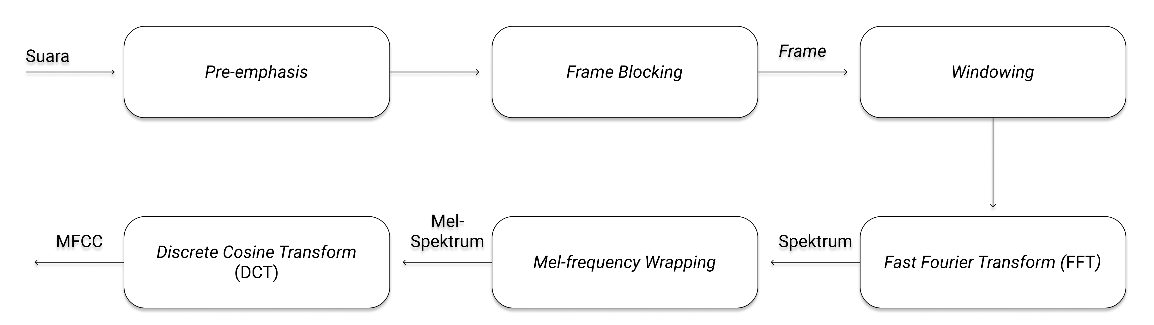
\includegraphics [width = 14cm, height= 5cm]{gambar/alir_mfcc}}
\caption{Diagram Alir \textit{Mel Frequency Cepstral Coefficient}}.
\label{alir_mfcc}
\end{figure}

\begin{enumerate}
\item \textit{Pre-emphasis}
\par Pada tahapan awal dalam menggunakan MFCC yaitu dengan \textit{pre-emphasis}. \textit{Pre-emphasis} dilakukan untuk mengurangi \textit{noise} karena sinyal suara yang didapat sering mengalami gangguan \textit{noise} \citep{heriyanto2018}. Dalam mengurangi efek samping saat mekanisme produksi suara, digunakanlah \textit{pre-emphasis} untuk menekan suara dengan frekuensi tinggi pada sinyal suara yang didapat. Fungsi lain \textit{pre-emphasis} dapat menguatkan puncak spektrum suara berfrekuensi tinggi \citep{efendi2019}. Secara matematis, \textit{pre-emphasis} dapat dirumuskan seperti pada persamaan berikut.

\begin{equation}
	y(n) = s(n) - as(n-1)
	\label{eqn1}
\end{equation}

\par Pada persamaan \ref{eqn1} dapat dijelaskan bahwa $y(n)$ adalah sinyal yang ditekan, $s(n)$ merupakan sinyal yang terdigitasi, serta $a$ adalah sebuah ketetapan filter \textit{pre-emhasis} atau sinyal yang diekstrak, dengan nilai 0.9 < $a$ < 1.0.

\item \textit{Frame blocking} dan \textit{Windowing}
\par Dalam menganalisis sinyal ucapan ke dalam bentuk \textit{frame} dibutuhkan tahap \textit{frame blocking} \citep{heriyanto2018}. Setelah sinyal ucapan melewati tahapan \textit{pre-emphasis} maka sinyal tersebut dibagi menjadi beberapa \textit{frame} dengan memuat N sampel sinyal pada masing-masing \textit{frame} dan \textit{frame} yang saling yang berdekatan akan dipisahkan sejauh M sampel \citep{laksono2018}. Setiap sampel dapat dibagi panjang \textit{frame} menjadi beberapa \textit{frame} berdasarkan waktu yang terletak di antara 20 ms hingga 40 ms \citep{laksono2018}. Di antara bagian-bagian \textit{frame} dengan \textit{frame} lainnya terdapat bagian yang bertumpang tindih atau yang disebut \textit{overlap}, hal ini berguna agar antar \textit{frame} saling berkesinambungan \citep{efendi2019}.

\par Untuk mencegah ketidaksinambungan sinyal suara dari ujung awal sampai ujung akhir dari proses \textit{frame blocking}, maka dilakukanlah \textit{windowing} \citep{efendi2019}. Tujuan dari \textit{windowing} adalah untuk mengurangi efek diskontinu pada ujung tiap \textit{frame} \citep{heriyanto2018}. Ada dua fungsi yang biasa digunakan yaitu \textit{Rectangular Window} dan \textit{Hamming Window} \citep{laksono2018}. Fungsi \textit{Rectangular Window} di tulis dalam persamaan \ref{eqn2} sebagai berikut.

\begin{equation}
	W = 
	\begin{cases}
		1 & 0 \le n \le N\\
		0 & L
	\end{cases}
	\label{eqn2}
\end{equation}

\par Fungsi di atas merupakan salah satu cara untuk menghindari diskontinu pada ujung \textit{window}, dengan cara meruncingkan sinyal menjadi nol atau dekat dengan nol, hal ini dapat mengurangi kesalahan yang terjadi \citep{laksono2018}. Lalu untuk Fungsi \textit{Hamming} sendiri dapat digambarkan seperti bentuk jendela dengan mempertimbangkan blok berikutnya di dalam rantai pemrosesan ekstraksi fitur serta menyatukan semua garis frekuensi yang terdekat \citep{laksono2018}. Fungsi \textit{Hamming} di tulis dalam persamaan \ref{eqn3} sebagai berikut.

\begin{equation}
	W(n) = 
	\begin{cases}
		0,54 - 0,46 \cos (\frac{2 \pi n}{N} - 1) & 0 \le n \le N-1\\
		0 & Otherwise
	\end{cases}
	\label{eqn3}
\end{equation}

\par Pada persamaan \ref{eqn3} dapat dijelaskan bahwa $W(n)$ merupakan \textit{Hamming Window}, jumlah dari sampel diinisialkan dengan $N$ dan $n$ menginisialkan pada sampel saat ini \citep{dua2018}. Lalu hasil persamaan \textit{Hamming Window} dikalikan dengan sinyal masukan/ \textit{innput} yang telah ditetapkan, perhitungan tersebut dapat dijelaskan pada persamaan \ref{eqn4} berikut ini \citep{laksono2018}.

\begin{equation}
	Y(n) = y(n) \times w(n)
	\label{eqn4}
\end{equation}

\par Pada persamaan \ref{eqn4} dapat dijelaskan bahwa $n$ merupakan banyaknya sampel tiap \textit{frame}, sinyal \textit{output} diwakilkan dengan $Y(n)$, sinyal \textit{input} diwakilkan dengan $y(n)$ dan $w(n)$ mewakilkan dari \textit{Hamming Window}.

\item \textit{Fast Fourier Transform} (FFT)
\par Untuk melakukan konversi sinyal dari domain waktu menjadi domain frekuensi dengan cepat digunakanlah \textit{Fast Fourier Transform} (FFT) \citep{efendi2019}. FFT berguna dalam mengubah konvolusi getaran celah suara dan respons yang didapat dari gelombang saluran suara dalam domain waktu \citep{laksono2018}. FFT sendiri dikembangkan karena suatu masalah dapat diselesaikan dengan mengubah atau memodelkan suatu permasalahan dalam representasi matematika dan mendapatkan keuntungan dalam segi efisiensi dibandingkan hal lainnya \citep{efendi2019}.

\item \textit{Mel-frequency Wrapping} 
\par Pada tahap ini spektrum yang dikeluarkan dari FFT di \textit{wrapping} sehingga menghasilkan \textit{mel-scale} agar resolusi frekuensi terhadap pendengaran manusia disesuaikan \citep{laksono2018}. Spektrum FFT memiliki nilai frekuensi yang sangat lebar, sehingga harus dipetakan ke dalam \textit{mel-scale} agar dapat mengetahui energi yang tersedia pada setiap titik dengan bantuan \textit{triangular} filter bank. Untuk mendapatkan batas-batas nilai tertinggi dan nilai terendah dari \textit{mel-scale} berdasarkan frekuensi suara dalam \textit{mel-frequency} pada setiap filter bank dihitung berdasarkan persamaan \ref{eqn5} berikut ini \citep{efendi2019}.

\begin{equation}
	mel = 2595 \log_{10} \Big(1 + \frac{f}{700}\Big)
	\label{eqn5}
\end{equation}

\par Pada persamaan \ref{eqn5} dapat dijelaskan bahwa $mel$ merupakan skala \textit{mel-frequency} dan frekuensi linear diwakilkan dengan $f$.

\item \textit{Discrete Cosine Transform} (DCT)
\par Tahap \textit{Discrete Cosine Transform} (DCT) digunakan untuk mengubah nilai koefisien \textit{mel-spectrum} menjadi ke domain waktu \citep{dua2018}.

\end{enumerate}

\section{\textit{Acoustic Model}}
\par Terdapat dua komponen utama pada sistem \textit{voice-to-text}, yang pertama adalah model akustik (\textit{acoustic model}) dan model bahasa (\textit{language model}). Model yang mengandung representasi statistik dari setiap suara yang berbeda dalam bentuk kata ataupun kalimat merupakan model akustik. Pada tiap-tiap representasi statistik tersebut dapat menentukan sebuah label yang disebut dengan suku kata (\textit{phonemes}) \citep{misbullah2020}. Model akustik memiliki dua tipe yang berbeda, yaitu \textit{phonemes} dan kata. Dua tipe tersebut diimplementasikan dengan berbagai metode seperti \textit{Hidden Markov Model} (HMM), \textit{Support Vector Machines} (SVM), \textit{Dynamic Bayesian Networks} (DBN) dan \textit{Artificial Neural Network} (ANN) \citep{gupta2016}. Sebagian besar sistem pengenalan suara saat ini menggunakan HMM untuk menangani variabilitas temporal ucapan lalu menggunakan \textit{Gaussian Mixture Models} (GMM) untuk menentukan seberapa baik status yang dihasilkan dari tiap HMM tersebut cocok dengan \textit{frame} atau \textit{short window of frames of coefficient} yang mewakili \textit{input} dari akustik \citep{hinton2012}. Cara alternatif yang terbaik untuk mengevaluasi kecocokan HMM dengan menggunakan \textit{Deep Neural Network} (DNN).

\subsection{\textit{Deep Neural Network} (DNN)}
\par DNN memiliki cara kerja dengan  mengambil beberapa koefisien dari frame sebagai masukannya dan menghasilkan keluaran berupa probabilitas posterior dari status HMM \citep{hinton2012}. \textit{Deep Neural Network} merupakan salah satu cabang dari \textit{machine learning} yang menggunakan konsep jaringan syaraf tiruan atau yang disebut dengan \textit{Neural Network} \citep{laksono2018}. DNN merupakan \textit{feed-forward}, \textit{feed-forward} itu sendiri adalah salah satu bagian di \textit{Artificial Neural Network} (ANN) yang memiliki lebih dari satu lapisan di \textit{hidden units} antara masukan atau keluarannya \citep{hinton2012}. Pada umumnya terdapat tiga struktur dari \textit{neural network}, yaitu \textit{input layer}, \textit{hidden layer} dan \textit{output layer}. Pada \textit{input layer} tiap \textit{node} merepresentasikan vektor untuk jumlah data \textit{input}, lalu pada \textit{hidden layer} memiliki fungsi untuk mengontrol apakah informasi dapat diketahui atau tidak dari \textit{input layer} yang akan diteruskan ke layer berikutnya dan yang terakhir setiap \textit{node} pada \textit{output layer} didefinisikan sebagai target dari kelas yang akan diprediksi \citep{misbullah2020}. DNN terbukti dapat mengungguli GMM dalam berbagai tolak ukur pengenalan ucapan serta terkadang dengan margin yang besar, karena DNN sendiri memiliki banyak \textit{hidden layer} dan dibuktikan dengan dilatih menggunakan metode baru \citep{hinton2012}. Penggambaran model umum dari DNN ditunjukkan seperti pada Gambar \ref{dnn_arsitektur}, di mana variasi proses, jumlah dan urutan \textit{hidden layer} tergantung pada arsitekturnya \citep{musiol2016}. 

\begin{figure}[H]
\centering
\shadowbox
{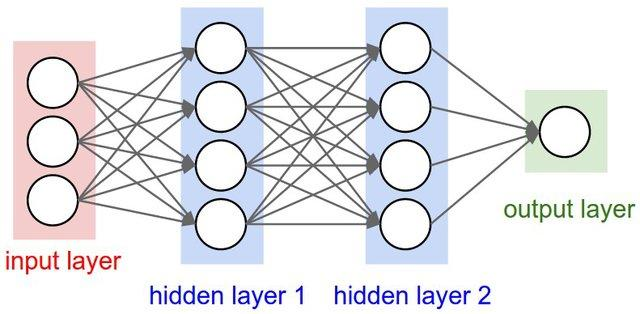
\includegraphics [width = 10cm, height= 5cm]{gambar/dnn_arsitektur}}
\caption{Model Umum dari \textit{Deep Neural Network} \citep{musiol2016}}.
\label{dnn_arsitektur}
\end{figure}

\par \textit{Neural Network} sendiri memiliki dua arsitektur, yaitu \textit{single layer perseptron} dan \textit{multi layer perseptron}. \textit{Single layer persepton} mempunyai satu \textit{hidden layer} yang digunakan, lalu pada \textit{multi layer perseptron} mempunyai lebih dari dua \textit{hidden layer} yang digunakan \citep{laksono2018}. Untuk mendapatkan hasil yang akurat, pada \textit{Deep Neural Network} atau \textit{Deep Learning} menggunakan jumlah \textit{hidden layer} yang sangat banyak \citep{laksono2018}.

\section{Kaldi \textit{Toolkit}}
Salah satu \textit{toolkit} untuk pengenalan suara yang \textit{open-source} adalah Kaldi, Kaldi sendiri ditulis dalam bahasa C++ dan di bawah lisensi Apache v2.0 \citep{povey2011}. Kaldi bergantung dengan dua \textit{library} dari luar yang tersedia secara bebas, \textit{library} yang pertama adalah OpenFst digunakan untuk \textit{finite-state framework} lalu untuk \textit{library} aljabar linear ekstensif menggunakan "\textit{Basic Linear Algebra Subrutin}" (BLAS) dan "\textit{Linear Algebra PACKage}" (LAPACK) \citep{povey2011}. Fitur pada Kaldi yang dapat digunakan adalah ekstraksi fitur yang paling umum digunakan, pemodelan akustik dengan beberapa model umum namun dapat diperluas dengan model jenis baru, \textit{phonetic decision tree} yang efisien untuk ukuran konteks arbitrer dan juga mendukung dengan berbagai pendekatan, pemodelan bahasa dapat menggunakan model bahasa apa pun yang dapat direpresentasikan sebagai \textit{finite-state transducer} (FST) serta dapat menggunakan \textit{toolkit} IRSTLM untuk membangun pemodelan Bahasa dari teks mentah, dan dapat membuat grafik decoding yang didasarkan pada \textit{Weighted Finite State Transducers} (WFSTs) \citep{povey2011}. Kaldi terus dikembangkan dan sedang mengerjakan model Bahasa yang besar dalam kerangka FST, pembuatan kisi dan pelatihan diskriminatif \citep{povey2011}.

\section{\textit{Indoor Positioning System}}
\textit{Indoor Positioning System} (IPS) dapat menemukan lokasi orang atau objek di dalam ruangan dengan menggunakan gelombang radio, medan magnet, sinyal akustik serta informasi sensoris yang dikumpulkan oleh alat teknologi berupa \textit{smartphone}, tablet, atau perangkat pintar lainnya \citep{atlas2016}. IPS memiliki beberapa pendekatan yaitu, \textit{positioning systems} berbasis WiFi (WPS), \textit{positioning systems} berbasis \textit{Bluetooth Low Energy} (BLE), sistem berbasis Identifikasi Frekuensi Radio (RFID) dan teknologi \textit{Ultra-Wide Band} (UWB) atau \textit{Visible Light Communication} (VLC) \citep{canton2017}.

\par \textit{Bluetooth Low Energy} (BLE) \textit{Beacon} merupakan suatu perangkat yang berukuran kecil dan menggunakan baterai sebagai sumber tenaganya, BLE dapat mengirimkan sinyal di area yang terbatas sampai 20 meter / 70 kaki dan bereaksi terhadap lokasi seseorang yang berada dalam jangkauan \citep{atlas2016}. BLE memiliki kelebihan yang dapat mengalahkan WPS yang telah popular dimasa lalu. BLE menawarkan harga yang lebih murah dan memiliki daya yang rendah, sehingga untuk infrastruktur yang tidak memungkinkan adanya WiFi dapat menjadi pilihan terbaik \citep{canton2017}. BLE dikenal sebagai pilihan yang terbaik karena mampu menyiarkan data menggunakan daya yang minimal hal itu didasarkan karena teknologi \textit{Bluetooth} yang digunakannya, serta BLE ideal untuk perangkat yang dapat berfungsi tanpa gangguan untuk jangka waktu yang lama karena menggunakan baterai kecil. Dari hal yang sudah dijelaskan sebelumnya BLE dapat berfungsi dengan baik untuk keperluan navigasi di dalam ruangan \citep{herrera2016}. 


%-----------------------------------------------------------------------------%

% Baris ini digunakan untuk membantu dalam melakukan sitasi
% Karena diapit dengan comment, maka baris ini akan diabaikan
% oleh compiler LaTeX.
\begin{comment}
\bibliography{daftar-pustaka}
\end{comment}
